\section{Theoretical Analysis} \label{section:theo}


\par In this section, a theoretical analysis of the circuit was conducted.

Initially, we used a transformer to transform Vs=230V in a smaller value (Vr=230/n with n=11)so that the rest of the circuit can aproximate it to 12 V. However, we want a DC voltage, not the initial AC voltage. In order to do achieve that, we use the circuit shown in Introduction.

1)The four diodes on the left are a full wave rectifier which means, they transform the AC current in an equal amplitude unidirectional current (blue plot). To compute that all we had to do was taking the the absolute value of the transformed voltage vr.



2)Then, a capacitor is used to reduce the magnitude of the voltage making it closer to a DC (orange plot). In order to compute this, we discovered when are the diodes ON and OFF . Periodically, if t$<$tOFF we got vO = vr and if t$>$tOFF we got 
\par vO = Vs*cos(w*tOFF)*exp(-(t-tOFF)/(Req*C)) due to the capacitor.The ripple voltage is basically max(vO)-min(vO). To make the next point clear vO will now be renamed vOenv.

\begin{table}[ht]
  \centering
  \begin{tabular}{|l|r|}
    \hline    
    {\bf Name} & {\bf Value} \\ \hline
    RippleEnvelope & 2.469091e-01 \\ \hline
AverageEnvelope & 2.078564e+01 \\ \hline

  \end{tabular}
  \caption{Ripple and average envelope values}
  \label{tab:p2}
\end{table}


3) Last, a series of 22 diodes reduce the noise making the current an almost perfect DC (green plot). Calculating the vO average from 2) we are able to see if the voltage difference between v5 and v0 is limited by the maximum voltage that the diodes can handle (this happens if the average is greater than that maximum). Right now, we have the voltage due to the DC ($dc_vO$) so we still need the voltage due to the AC. It is possible to compute that calculating rD which is the resistance of each diode and 

\par $acvO = num_diodes*rD/(numdiodes*rd+R2) * (vOenv-averageenv)$. 

\par In the end, $vO$= $ac_vO$ + $dcvO$. The average must be aproximadetly 12V.

\begin{table}[ht]
  \centering
  \begin{tabular}{|l|r|}
    \hline    
    {\bf Name} & {\bf Value} \\ \hline
    RippleRegulator & 7.200294e-03 \\ \hline
AverageRegulator& 1.200006e+01 \\ \hline

  \end{tabular}
  \caption{Ripple and average regulator values}
  \label{tab:p2}
\end{table}


The figure shows the plots mentioned above.

\begin{figure}[h] \centering
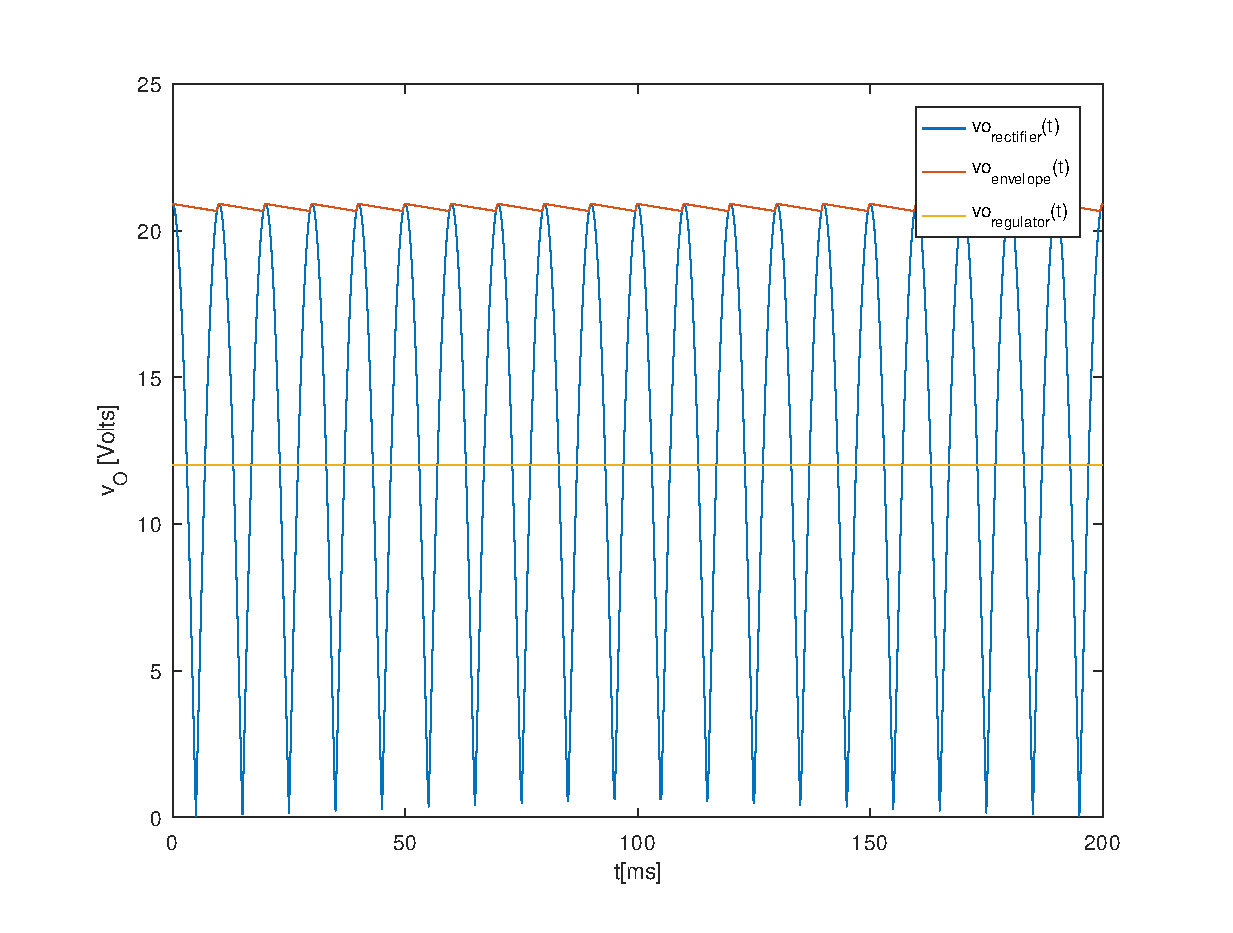
\includegraphics[width=0.65\linewidth]{all_vout.eps}
\caption{Input voltage of the secundary circuit (v(2)), output Voltage of the Envelope Detector (v(4)), Voltage Regulator (v(5)), and v(5)-12}
\label{sim3}
\end{figure}


\begin{figure}[h] \centering
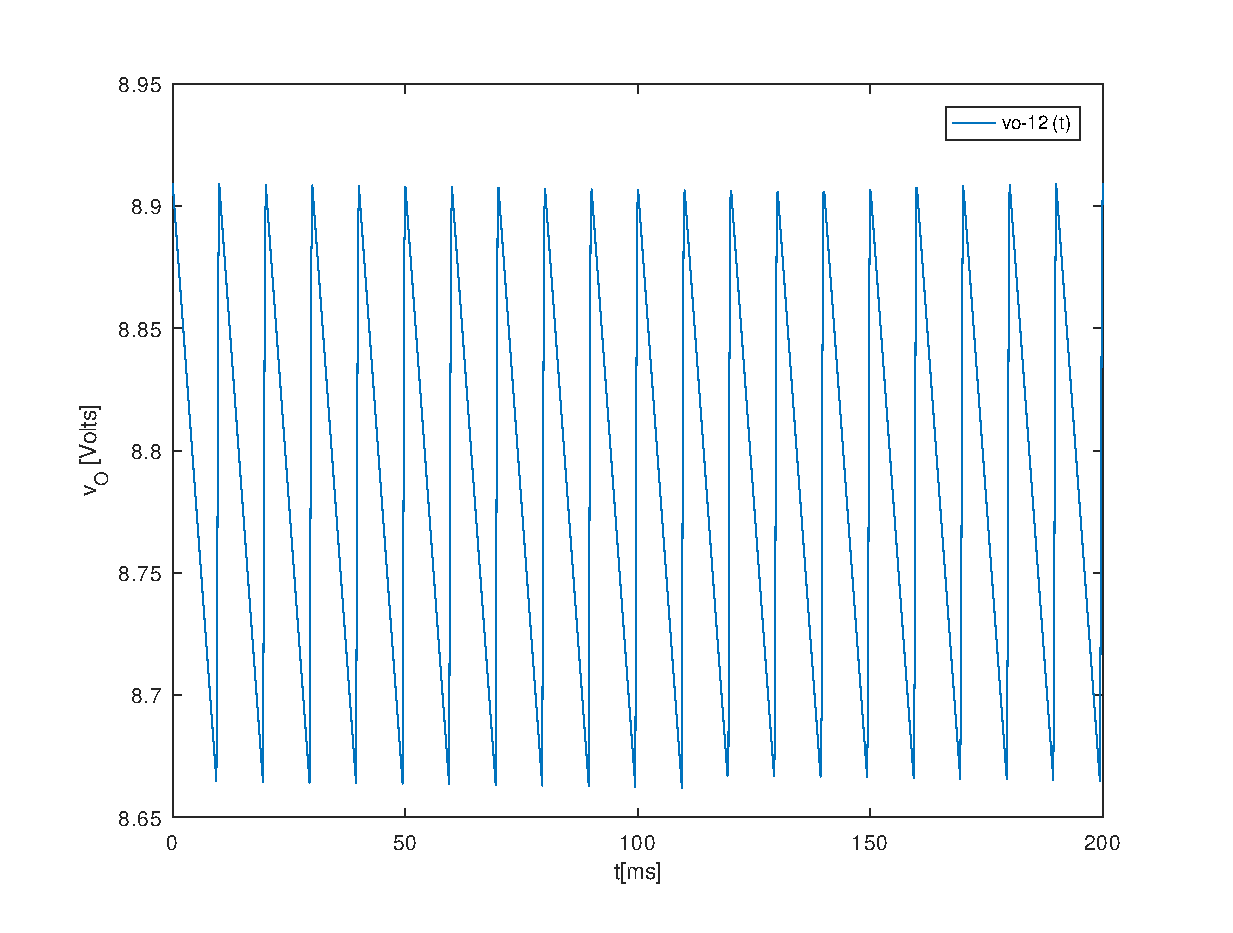
\includegraphics[width=0.65\linewidth]{deviation.eps}
\caption{Output AC components + DC deviation}
\label{sim3}
\end{figure}
















